% Generated by extension/spectral_transfer/make_scale_assets.py. Do not edit.
\definecolor{pairexact}{HTML}{217D91}
\definecolor{closedcol}{HTML}{A64442}
\definecolor{donorcol}{HTML}{5D6670}
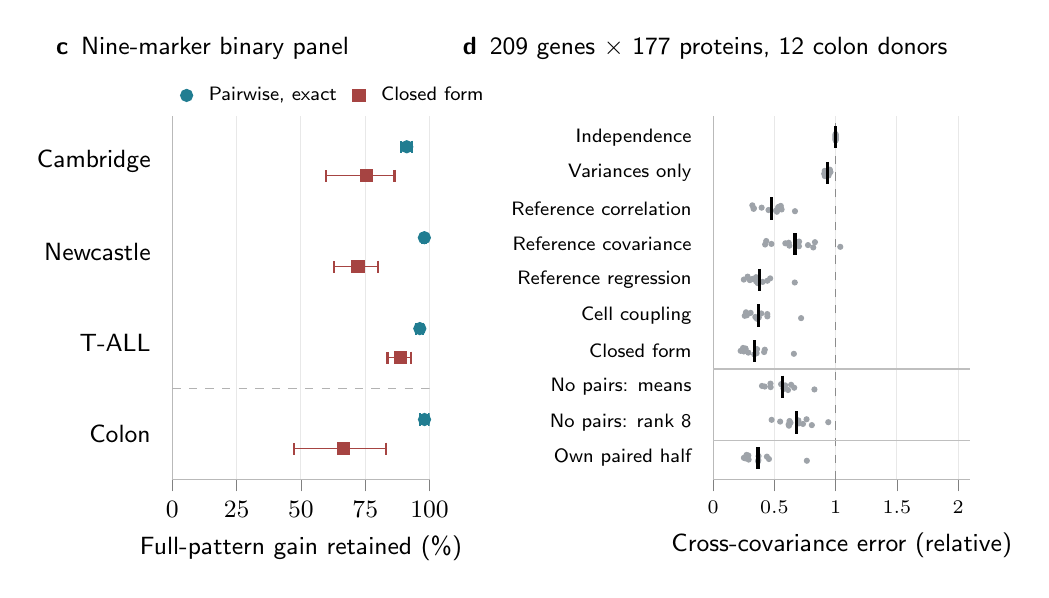
\begin{tikzpicture}[font=\sffamily]
\begin{axis}[name=left,
 width=.40\textwidth,height=6.2cm,
 xmin=0,xmax=100,ymin=.5,ymax=4.5,
 xtick={0,25,50,75,100},ytick={1,2,3,4},yticklabels={Colon,T-ALL,Newcastle,Cambridge},
 xlabel={Full-pattern gain retained (\%)},
 title={\textbf{c}\enspace Nine-marker binary panel},
 title style={font=\sffamily\small,at={(0,1)},anchor=south west,xshift=-1.6cm,yshift=11pt},
 axis x line*=bottom,axis y line*=left,tick align=outside,y tick style={draw=none},
 xmajorgrids=true,grid style={gray!18},axis line style={gray!55},
 tick label style={font=\sffamily\small},label style={font=\sffamily\small},
 legend style={draw=none,at={(0,1.0)},anchor=south west,font=\sffamily\scriptsize,legend columns=2,column sep=4pt},
 every axis plot/.append style={only marks,mark size=2pt,line width=.75pt},
 error bars/x dir=both,error bars/x explicit,
 error bars/error mark options={rotate=90,mark size=2.2pt,line width=.75pt}]
\draw[dashed,black!30] (axis cs:0,1.5) -- (axis cs:100,1.5);
\addplot[color=pairexact,mark=*] coordinates { (91.124,4.16) += (1.898,0) -= (2.193,0) (97.964,3.16) += (0.814,0) -= (0.909,0) (96.205,2.16) += (1.230,0) -= (1.585,0) (98.024,1.16) += (1.816,0) -= (1.798,0) };
\addlegendentry{Pairwise, exact}
\addplot[color=closedcol,mark=square*] coordinates { (75.316,3.84) += (11.052,0) -= (15.573,0) (72.180,2.84) += (7.857,0) -= (9.317,0) (88.774,1.84) += (4.005,0) -= (5.133,0) (66.426,0.84) += (16.748,0) -= (19.207,0) };
\addlegendentry{Closed form}
\end{axis}
\begin{axis}[at={(left.east)},anchor=west,xshift=3.6cm,
 width=.40\textwidth,height=6.2cm,
 xmin=0,xmax=2.1,ymin=.4,ymax=10.6,
 xtick={0,.5,1,1.5,2},ytick={1,2,3,4,5,6,7,8,9,10},yticklabels={{Own paired half},{No pairs: rank 8},{No pairs: means},{Closed form},{Cell coupling},{Reference regression},{Reference covariance},{Reference correlation},{Variances only},{Independence}},
 xlabel={Cross-covariance error (relative)},
 title={\textbf{d}\enspace 209 genes $\times$ 177 proteins, 12 colon donors},
 title style={font=\sffamily\small,at={(0,1)},anchor=south west,xshift=-3.3cm,yshift=11pt},
 axis x line*=bottom,axis y line*=left,tick align=outside,y tick style={draw=none},
 xmajorgrids=true,grid style={gray!18},axis line style={gray!55},
 tick label style={font=\sffamily\scriptsize},label style={font=\sffamily\small},clip=false]
\draw[dashed,black!45] (axis cs:1,.4) -- (axis cs:1,10.6);
\draw[black!25] (axis cs:0,1.5) -- (axis cs:2.1,1.5);
\draw[black!25] (axis cs:0,3.5) -- (axis cs:2.1,3.5);
\addplot[only marks,mark=*,mark size=.9pt,color=donorcol!60] coordinates {
 (0.3673,0.910) (0.7653,0.926) (0.3696,0.943) (0.2904,0.959) (0.4560,0.975) (0.2635,0.992) (0.2514,1.008) (0.2724,1.025) (0.4394,1.041) (0.3713,1.057) (0.2878,1.074) (0.2733,1.090)
 (0.6194,1.910) (0.8059,1.926) (0.6166,1.943) (0.7338,1.959) (0.7008,1.975) (0.6317,1.992) (0.9401,2.008) (0.5475,2.025) (0.6239,2.041) (0.6963,2.057) (0.4779,2.074) (0.7628,2.090)
 (0.6117,2.910) (0.8271,2.926) (0.5788,2.943) (0.5741,2.959) (0.6621,2.975) (0.4700,2.992) (0.4218,3.008) (0.3993,3.025) (0.5884,3.041) (0.6368,3.057) (0.5552,3.074) (0.4685,3.090)
 (0.3360,3.910) (0.6595,3.926) (0.3555,3.943) (0.2880,3.959) (0.4167,3.975) (0.2509,3.992) (0.2253,4.008) (0.2666,4.025) (0.4221,4.041) (0.3588,4.057) (0.2650,4.074) (0.2449,4.090)
 (0.3577,4.910) (0.7184,4.926) (0.3730,4.943) (0.3450,4.959) (0.4432,4.975) (0.2587,4.992) (0.2762,5.008) (0.2684,5.025) (0.4423,5.041) (0.3932,5.057) (0.3067,5.074) (0.2687,5.090)
 (0.3644,5.910) (0.6667,5.926) (0.4047,5.943) (0.3515,5.959) (0.4428,5.975) (0.3003,5.992) (0.2512,6.008) (0.3204,6.025) (0.4662,6.041) (0.3618,6.057) (0.3504,6.074) (0.2820,6.090)
 (0.8178,6.910) (1.0382,6.926) (0.7007,6.943) (0.6228,6.959) (0.7747,6.975) (0.4249,6.992) (0.4763,7.008) (0.5898,7.025) (0.6172,7.041) (0.8314,7.057) (0.7018,7.074) (0.4338,7.090)
 (0.5209,7.910) (0.6684,7.926) (0.5133,7.943) (0.4525,7.959) (0.5595,7.975) (0.3307,7.992) (0.3332,8.008) (0.3964,8.025) (0.5316,8.041) (0.5435,8.057) (0.5529,8.074) (0.3204,8.090)
 (0.9121,8.910) (0.9425,8.926) (0.9151,8.943) (0.9325,8.959) (0.9068,8.975) (0.9431,8.992) (0.9488,9.008) (0.9583,9.025) (0.9531,9.041) (0.9111,9.057) (0.9523,9.074) (0.9527,9.090)
 (1.0000,9.910) (1.0000,9.926) (1.0000,9.943) (1.0000,9.959) (1.0000,9.975) (1.0000,9.992) (1.0000,10.008) (1.0000,10.025) (1.0000,10.041) (1.0000,10.057) (1.0000,10.074) (1.0000,10.090)};
\addplot[only marks,mark=|,mark size=4pt,line width=1.2pt,color=black] coordinates { (0.3673,1) (0.6797,2) (0.5662,3) (0.3408,4) (0.3710,5) (0.3802,6) (0.6691,7) (0.4769,8) (0.9357,9) (1.0000,10) };

\end{axis}
\end{tikzpicture}
